\documentclass[journal,12pt,twocolumn]{IEEEtran}
\IEEEoverridecommandlockouts
\usepackage{cite}
\usepackage{amsmath,amssymb,amsfonts,bm}
\usepackage{mathtools}
\usepackage{tkz-euclide} 
\usepackage{tikz}
\usetikzlibrary{calc,math}
 \usepackage{caption}
\usepackage{listings}
\usepackage{gensymb}
\let\vec\mathbf
\numberwithin{equation}{subsection}

\newcommand{\myvec}[1]{\ensuremath{\begin{pmatrix}#1\end{pmatrix}}}
\newcommand{\norm}[1]{\left\lVert#1\right\rVert}
\newcommand{\mydet}[1]{\ensuremath{\begin{vmatrix}#1\end{vmatrix}}}

\renewcommand\thesection{\arabic{section}}
\renewcommand\thesubsection{\thesection.\arabic{subsection}}
\renewcommand\thesubsubsection{\thesubsection.\arabic{subsubsection}}

\renewcommand\thesectiondis{\arabic{section}}
\renewcommand\thesubsectiondis{\thesectiondis.\arabic{subsection}}
\renewcommand\thesubsubsectiondis{\thesubsectiondis.\arabic{subsubsection}}
%\renewcommand{\theequation}{\theenumi}
%\numberwithin{equation}{enumi}

\providecommand{\mbf}{\mathbf}
\providecommand{\pr}[1]{\ensuremath{\Pr\left(#1\right)}}
\providecommand{\qfunc}[1]{\ensuremath{Q\left(#1\right)}}
\providecommand{\sbrak}[1]{\ensuremath{{}\left[#1\right]}}
\providecommand{\lsbrak}[1]{\ensuremath{{}\left[#1\right.}}
\providecommand{\rsbrak}[1]{\ensuremath{{}\left.#1\right]}}
\providecommand{\brak}[1]{\ensuremath{\left(#1\right)}}
\providecommand{\lbrak}[1]{\ensuremath{\left(#1\right.}}
\providecommand{\rbrak}[1]{\ensuremath{\left.#1\right)}}
\providecommand{\cbrak}[1]{\ensuremath{\left\{#1\right\}}}
\providecommand{\lcbrak}[1]{\ensuremath{\left\{#1\right.}}
\providecommand{\rcbrak}[1]{\ensuremath{\left.#1\right\}}}

\lstset{
frame=single, 
breaklines=true,
columns=fullflexible
}

\begin{document}

\title{Matrix Theory EE5609 - Assignment 5\\
}

\author{\IEEEauthorblockN{Sandhya Addetla}\\
\IEEEauthorblockA{PhD Artificial Inteligence Department} \\
AI20RESCH14001\\
 }

\maketitle
\begin{abstract}
 Find the asymptotes of the given hyperbola and also the equation to its conjugate hyperbola
\end{abstract}

Download all python codes from 
\begin{lstlisting}
https://github.com/SANDHYA-A/Assignment5/blob/master/Assignment5.py
\end{lstlisting}

\section{Problem Statement}
 Find the asymptotes of the given hyperbola and also the equation to its conjugate hyperbola
\begin{align}
19x^2 + 24xy+y^2-22x-6y=0 \label{1.1}
\end{align}
\section{Solution}
The general equation of second degree is given by
\begin{align}
ax^2+2bxy+cy^2+2dx+2ey+f=0\label{2.1}
\end{align}
and can be expressed as
\begin{align}
\vec{x}^T\vec{V}\vec{x}+2\vec{u}^T\vec{x}+f=0 \label{2.2}
\end{align}
where
\begin{align}
\vec{V} &= \vec{V}^T = \myvec{a & b \\ b & c}
\\
\vec{u} &= \myvec{d \\ e}
\intertext{Comparing equations \ref{1.1} and \ref{2.2} we get}
    \vec{V}=\vec{V}^T&=\myvec{19 & 12 \\ 12 &1}\label{2.5}\\
    \vec{u}&=\myvec{-11 \\-3 }\label{2.6}\\
    f&=0\label{2.7}
\end{align}   
Expanding the Determinant of $\vec{V}$.
\begin{align}
    \Delta_{V} &= \begin{array}{|cc|}
19 &12\\12 & 1
\end{array}<0\label{2.8}
\end{align}
Hence from \ref{2.8} given
equation represents the hyperbola.\\
The characteristic equation of $\vec{V}$ is obtained by evaluating the determinant 
\begin{align}
       \begin{array}{|c|}
V-\lambda\vec{I}
\end{array}&=0\\
   \begin{array}{|cc|}
19-\lambda & 12 \\ 12 & 1-\lambda
\end{array}&=0\\
    \brak{19-\lambda}\brak{1-\lambda}-144=0\\
    \lambda_{1}=-5,   \lambda_{2}= 25 \label{2.12}
\end{align}
The eigenvector $\vec{p}$ is defined as 
\begin{align}
    \vec{V}\vec{p}&=\lambda\vec{p}\\
    \implies (\vec{V}-\lambda\vec{I})\vec{p}&=0\label{2.14}
\end{align}
For $\lambda_1=-5$ ,
\begin{align}
    (\vec{V}-\lambda_1\vec{I})=\myvec{19+5 & 12 \\12 & 1+5}
\end{align}
By row reduction , 
\begin{align}
    &\myvec{24 & 12 \\12 & 6}\\
&\xleftrightarrow{R_2\leftarrow 2R_2 -R_1}
    \myvec{24 & 12 \\ 0& 0}\\
        &\xleftrightarrow{R_1\leftarrow \frac{R_1}{12}}
    \myvec{2 & 1 \\ 0& 0}
    \label{2.18}
\end{align}
Subsituting equation \ref{2.18} in equation \ref{2.14} we get
\begin{align}
        &   \myvec{2 & 1 \\ 0& 0}\myvec{u_1 \\ u_2}=\myvec{0 \\ 0}\label{2.19}
\end{align}
Where, $\vec{p}=\myvec{u_1\\u_2}$
Let $u_1=t$
\begin{align}
    u_2&=-2t
\end{align}
Eigen vector $\vec{p_1}$ is given by
\begin{align}
    \vec{p_1}&=\myvec{t \\ -2t}
\end{align}
Let $t=1$, we get
\begin{align}
        \vec{p_1}&=\myvec{1 \\-2 }\label{2.22}
\end{align}
For $\lambda_2=25$ ,
\begin{align}
    (\vec{V}-\lambda_2\vec{I})=\myvec{19-25 & 12 \\12 & 1-25}
\end{align}
By row reduction , 
\begin{align}
    &\myvec{-6 & 12 \\12 & -24}\\
&\xleftrightarrow{R_2\leftarrow R_2 +2R_1}
    \myvec{-6 & 12 \\ 0& 0}\\
        &\xleftrightarrow{R_1\leftarrow \frac{R_1}{6}}
    \myvec{-1 & 2 \\ 0& 0}
    \label{2.26}
\end{align}
Subsituting equation \ref{2.26} in equation \ref{2.14} we get
\begin{align}
        &   \myvec{-1 & 2 \\ 0& 0}\myvec{v_1 \\ v_2}=\myvec{0 \\ 0}\label{2.27}
\end{align}
Where, $\vec{p}=\myvec{v_1\\v_2}$
Let $v_1=t$
\begin{align}
    v_2&=\frac{t}{2}
\end{align}
Eigen vector $\vec{p_2}$ is given by
\begin{align}
    \vec{p_2}&=\myvec{t \\ \frac{t}{2}}
\end{align}
Let $t=1$, we get
\begin{align}
        \vec{p_2}&=\myvec{1 \\\frac{1 }{2}}\label{2.30}
\end{align}
By eigen decompostion $\vec{V}$ can be represented by
\begin{align}
    \vec{V}&=\vec{P}\vec{D}\vec{P}^T\label{2.31}
\end{align}
where 
\begin{align}
        \vec{P}&=\myvec{\vec{p_1} & \vec{p_2}}\label{2.32}\\
    \vec{D}&=\myvec{\lambda_1 & 0 \\0 & \lambda_2}\label{2.33}
\end{align}

Substituting equations \ref{2.22}, \ref{2.30} in equation \ref{2.32} we get 
\begin{align}
    \vec{P}&=\myvec{1 & 1 \\-2 & \frac{1}{2}}\label{2.34}
\end{align}
Substituting equation \ref{2.12} in \ref{2.33} we get
\begin{align}
       \vec{D}&=\myvec{-5 & 0\\0 & 25}\label{2.35}
\end{align}
Equation of a hyperbola and the combined equation of the Asymptotes differ only in the constant term.
\begin{align}
 19x^2 + 24xy+y^2-22x-6y+K=0   \label{2.36}
\end{align}
The above equation can be expressed in the form 
\begin{align}
\vec{x}^T\vec{V}\vec{x}+2\vec{u}^T\vec{x}+f&=0 \label{2.37}
\intertext{Comparing equation we get}
    \vec{V}=\vec{V}^T&=\myvec{19 & 12 \\ 12 &1}\label{2.38}\\
    \vec{u}&=\myvec{-11 \\-3 }\label{2.39}\\
    f&=K\label{2.40}
\end{align}
\begin{align}
\Delta&=\begin{array}{|ccc|}19 & 12 & -11\\ 12& 1 & -3\\ -11 & -3 & K
\end{array}
\end{align}
Since the equations represent pair of straight lines, equating the determinant to zero, we can get the value of K
\begin{align}
\implies K=4 \label{2.42}
\end{align}
Let $(\alpha,\beta)$ be their point of intersection, then
\begin{equation}\label{2.43}
	\myvec{ a & b\\ b & c}\myvec{\alpha \\ \beta} = \myvec{-d \\ -e}
\end{equation}
Substituting the values, we obtain,
\begin{align}
\myvec{19 & 12 \\ 12 &1}\myvec{\alpha \\ \beta} = \myvec{11 \\ 3}\\
\text{We get, } \alpha =  \frac{1}{5} , \beta = \frac{3}{5}
\end{align}

Using Affine transformation and Spectral decomposition, we get
\begin{align}
X^\prime = \pm \sqrt{-\frac{\lambda_2}{\lambda_1}}Y^\prime\\
\text{where } X^\prime = Xu_1 + Yu_2 \\
Y^\prime = Xv_1 + Yv_2\\
X = x-\alpha \text{ and } Y = y - \beta
\end{align}
Therefore, 
\begin{multline}
	u_1(x-\alpha) + u_2(y-\beta) = \\ \pm \sqrt{-\frac{\lambda_2}{\lambda_1}}(v_1(x-\alpha) + v_2(y-\beta))  \label{2.57}
\end{multline}
Substituting values, we get 
\begin{multline}
	(x-\frac{1}{5})-2(y-\frac{3}{5}) = \\ \pm \sqrt{\frac{25}{5}}(x-\frac{1}{5})+\frac{1}{2}(y-\frac{3}{5}) 
\end{multline}
Simplifying above equation
\begin{align}
	8x+ 9y - 7 = 0 \\
	12x + y + 7 = 0\\
	\implies (8x+ 9y - 7 )(12x + y + 7) = 0
\end{align}
Thus the equation of lines are
\begin{align}
	\myvec{8 & 9}\vec{x} = 7 \\
	\myvec{12 & 1}\vec{x} = -7 
\end{align}

 The Equation of Conjugate hyperbola is given by:\\
\\
2(Equation of Asymptotes)- Equation of hyperbola.\\
\\
From Eq \ref{1.1} and \ref{2.36}, we obtain equation of Conjugate hyperbola as:-
\begin{align}
19x^2 + 24xy+y^2-22x-6y+8=0  \label{2.57}
\end{align}
The general equation of second degree is given by
\begin{align}
ax^2+2bxy+cy^2+2dx+2ey+f=0\label{2.59}
\end{align}
comparing equation \ref{2.57} with the general equation of second degree given at \ref{2.59}, it can be expressed as
\begin{align}
\vec{x}^T\vec{V}\vec{x}+2\vec{u}^T\vec{x}+f=0 \label{2.58}
\end{align}
where
\begin{align}
\vec{V} &= \vec{V}^T = \myvec{a & b \\ b & c}
\\
\vec{u} &= \myvec{d\\ e}
\intertext{Comparing equations \ref{2.57} and \ref{2.58} we get}
    \vec{V}=\vec{V}^T&=\myvec{19 & 12 \\ 12 &1}\\
    \vec{u}&=\myvec{-11 \\-3 }\\
    f&=8
\end{align}   
Therefore, the equation of the conjugate hyperbola is as given below:-
\begin{align}
\vec{x}^T\myvec{19 & 12 \\12 & 1}\vec{x} +2\myvec{-11 & -3} \vec{x}&+8= 0 \label{2.66}
\end{align}

\begin{figure}[h]
    \centering
    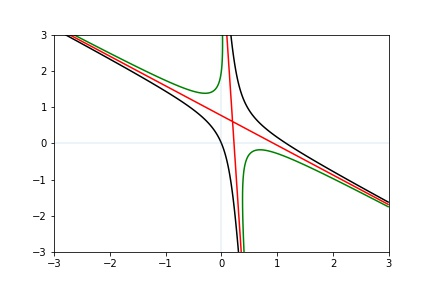
\includegraphics[width=\columnwidth]{hyperbola.jpg}
    \caption{Hyperbola, Conjugate Hyperbola and Asymptotes}
    \label{Fig :1}
\end{figure}
\end{document}